% fig_goose_timing.tex
% GOOSE transfer sequence timing diagram (TR-14)
% Shows: DS_CLOSE, DS_OPEN, GOOSE latency, zone reconfiguration point
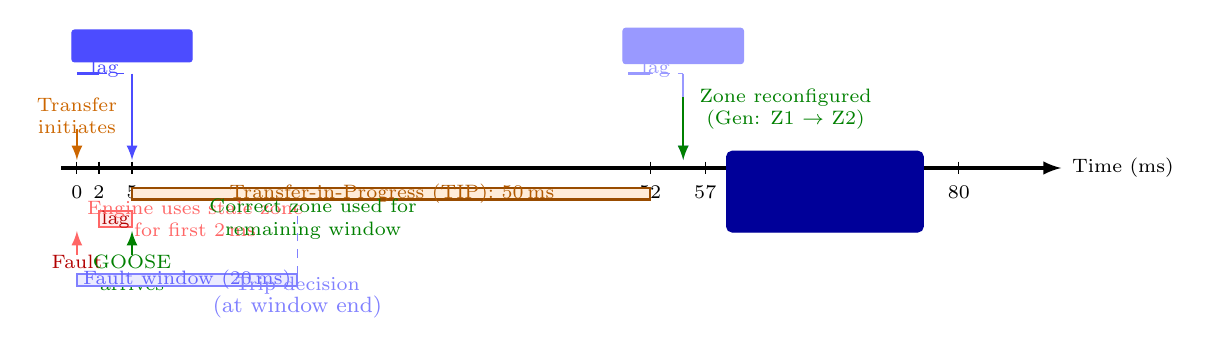
\begin{tikzpicture}[
  event/.style={draw, fill=white, rounded corners=1pt,
                font=\scriptsize, minimum width=36pt, minimum height=11pt},
  tline/.style={very thick},
  arrow/.style={-latex, thick},
  lab/.style={font=\scriptsize},
  ]

% ---- Time axis -------------------------------------------------------------
\draw[tline, -latex] (-0.2, 0) -- (12.5, 0) node[right, lab]{Time (ms)};
% Tick marks
\foreach \t/\tlab in {0/0, 2/2, 5/5, 52/52, 57/57, 80/80} {
  \draw (\t*0.14, 0.08) -- (\t*0.14, -0.08);
  \node[lab, below] at (\t*0.14, -0.10) {\tlab};
}

% ---- Transfer initiation ---------------------------------------------------
\draw[arrow, orange!80!black] (0, 0.5) -- (0, 0.10)
  node[above=6pt, lab, align=center, orange!80!black]{Transfer\\initiates};

% ---- DS_CLOSE signal -------------------------------------------------------
\draw[thick, blue!70] (0, 1.2) -- (0.28, 1.2);
\draw[dashed, blue!70] (0.28, 1.2) -- (0.70, 1.2);   % 2 ms lag
\draw[thick, blue!70, -latex] (0.70, 1.2) -- (0.70, 0.10);
\node[event, blue!70] at (0.70, 1.55) {DS2 closes};
\node[lab, blue!70, align=center] at (0.35, 1.40) {2\,ms\\lag};

% ---- TIP state bar ---------------------------------------------------------
\fill[orange!15] (0.70, -0.4) rectangle (7.28, -0.25);
\draw[orange!60!black, thick] (0.70, -0.4) rectangle (7.28, -0.25);
\node[lab, orange!70!black] at (4.0, -0.32) {Transfer-in-Progress (TIP):  50\,ms};

% ---- DS_OPEN signal --------------------------------------------------------
\draw[thick, blue!40] (7.28, 1.2) -- (7.00, 1.2);    % DS1 opens after 50ms
\draw[dashed, blue!40] (7.00, 1.2) -- (7.70, 1.2);   % 2 ms lag
\draw[thick, blue!40, -latex] (7.70, 1.2) -- (7.70, 0.10);
\node[event, blue!40] at (7.70, 1.55) {DS1 opens};
\node[lab, blue!40, align=center] at (7.35, 1.40) {2\,ms\\lag};

% ---- Zone reconfiguration --------------------------------------------------
\draw[thick, green!50!black, -latex] (7.70, 0.90) -- (7.70, 0.10);
\node[lab, green!50!black, align=center] at (9.0, 0.75)
  {Zone reconfigured\\(Gen: Z1 $\to$ Z2)};

% ---- Fault window (T5_LAG scenario) ----------------------------------------
\fill[red!8] (0.28, -0.75) rectangle (0.70, -0.55);   % lag window (0-2ms)
\draw[red!60, thick] (0.28, -0.75) rectangle (0.70, -0.55);
\node[lab, red!70!black] at (0.49, -0.65) {lag};

% Fault occurs at t=0 (before DS_CLOSE received)
\draw[arrow, red!60] (0, -1.1) -- (0, -0.80)
  node[below=5pt, lab, red!70!black]{Fault};
\node[lab, red!60, align=center] at (1.5, -0.65)
  {\scriptsize Engine uses stale zone\\for first 2\,ms};

% After GOOSE update:
\draw[arrow, green!50!black] (0.70, -1.1) -- (0.70, -0.80)
  node[below=5pt, lab, green!50!black, align=center]{GOOSE\\arrives};
\node[lab, green!50!black, align=center] at (3.0, -0.65)
  {\scriptsize Correct zone used for\\remaining window};

% ---- Relay decision window --------------------------------------------------
\fill[blue!8] (0, -1.5) rectangle (2.80, -1.35);
\draw[blue!50, thick] (0, -1.5) rectangle (2.80, -1.35);
\node[lab, blue!60] at (1.40, -1.42) {Fault window (20\,ms)};

\draw[blue!50, dashed] (2.80, -1.35) -- (2.80, -0.55);

\node[lab, blue!50, align=center] at (2.80, -1.65)
  {Trip decision\\\footnotesize (at window end)};

% ---- Result annotation ------------------------------------------------------
\node[draw, fill=green!8, rounded corners=2pt, font=\scriptsize,
      align=center, blue!60!black]
  at (9.5, -0.30) {Correct trip\\even with 2\,ms lag\\(14/20\,ms valid)};

\end{tikzpicture}
